\chapter{世界面、威克轉動與道對偶}

\lectureoverview{粒子沿著世界線運動；弦則掃出一個世界面。將任一物體量子化，都需要對所有可能的歷史求和，但洛侖茲時空中的求和帶有振盪相位，難以定義。將世界面時間轉為虛座標後，便得到由拉普拉斯方程支配的歐幾里得理論。其共形對稱性接著可將四弦交互作用的帶縫曲面映成帶有四個邊界插入點的圓盤，讓直接道與交叉道之間的對稱性顯現出來。}

\section{從世界線到對所有歷史求和}

先從一個自由粒子談起。在非相對論力學中，粒子的位置是函數\(\mathbf x(t)\)；將質量設為 1 後，其作用量為
\begin{equation}
  S_{\mathrm{NR}}[\mathbf x]
  =\frac12\int_{t_1}^{t_2}\dot{\mathbf x}^{\,2}\,dt.
  \label{eq:l07-nr-action}
\end{equation}
對相對論性描述而言，更自然的做法是將時間和空間納入同一個向量\(X^\mu(\tau)\)，並以\(\tau\)作為沿軌跡的參數。相應的二次形式為
\begin{equation}
  S_{\mathrm{rel}}[X]
  =\frac12\int_{\tau_1}^{\tau_2}
  \frac{dX^\mu}{d\tau}\frac{dX_\mu}{d\tau}\,d\tau.
  \label{eq:l07-rel-action}
\end{equation}
上下指標反映了時間與空間之間的洛侖茲號差。
\editorialnote{此處使用的是固定世界線參數化下的二次相對論作用量。另一種明確具有重參數化不變性的形式，則正比於固有長度；講座稍後會提到這一點。}

\begin{figure}[H]
  \centering
  \includegraphics[width=0.72\textwidth]{lecture_07_figure_01.png}
  \caption{黑板上並列寫出非相對論作用量及其相對論二次形式。}
  \lectureframe{00:03:35}
  \label{fig:l07-particle-actions}
\end{figure}

在經典力學中，固定端點後對路徑作變分。自由粒子便沿著速度恆定的直線世界線運動。量子力學問的則是另一個問題：它不會在兩個端點之間選出一條軌跡，而是要問粒子從一點出發、並在另一點被探測到的振幅。每一條中間路徑都會貢獻一個相位，
\begin{equation}
  K(2,1)=\int_{X(1)}^{X(2)}\!\mathcal D X\,
  e^{iS[X]}.
  \label{eq:l07-feynman-integral}
\end{equation}
泛函積分是對無限維路徑空間所作的積分，並非作用量中已出現的普通積分。

\begin{figure}[H]
  \centering
  \includegraphics[width=0.72\textwidth]{lecture_07_figure_02.png}
  \caption{對所有軌跡求和之前，一條代表性路徑及其所帶的相位。}
  \lectureframe{00:06:21}
  \label{fig:l07-path-integral-board}
\end{figure}

用相對論的語言來說，這個點到點的振幅就是傳播子。在交互作用中，數段世界線會在某處相接。將各段的作用量相加，對相接點積分，再對符合外部粒子要求的圖形求和。因此，熟悉的費曼圖展開，其實已隱含在對所有歷史求和的指示之中。

此處以符號\(S\)表示作用量。它與熵無關，也與講座接近尾聲時使用的曼德斯塔姆變數\(s\)無關。兩者沿用相同記號只是傳統如此，並沒有特別的啟發性。

\section{將時間轉向側面}

\eqref{eq:l07-feynman-integral}有個立即浮現的問題。每個因子\(e^{iS}\)的絕對值都是 1。因此，劇烈振盪的軌跡和經典直線的絕對權重相同，兩者只有相位不同。相消干涉會讓經典行為重新顯現，但不會因此使形式上的積分成為普通的收斂積分。

引入新的參數\(s\)，令
\begin{equation}
  \tau=\alpha s,
  \qquad
  d\tau=\alpha\,ds,
  \qquad
  \frac{dX}{d\tau}=\frac{1}{\alpha}\frac{dX}{ds}.
\end{equation}
如此一來，二次作用量會按下式重新縮放：
\begin{equation}
  \frac12\int d\tau
  \left(\frac{dX}{d\tau}\right)^2
  =
  \frac{1}{2\alpha}\int ds
  \left(\frac{dX}{ds}\right)^2.
  \label{eq:l07-rescaled-action}
\end{equation}
選取對應於\(\alpha=-i\)的積分路徑後，振盪權重便轉為
\begin{equation}
  e^{iS}
  \longrightarrow
  \exp\!\left[-\frac12\int ds
  \left(\frac{dX}{ds}\right)^2\right]
  =e^{-S_E}.
  \label{eq:l07-euclidean-particle}
\end{equation}

\begin{figure}[H]
  \centering
  \includegraphics[width=0.66\textwidth]{lecture_07_figure_03.png}
  \caption{代入虛時間後的歐幾里得粒子權重；指數為實數且不大於零。}
  \lectureframe{00:16:20}
  \label{fig:l07-particle-wick}
\end{figure}

跑到很遠再折返，或是沒有走遠卻快速來回擺動的路徑，都會有很大的正\(S_E\)，因而受到指數抑制。所得的是一種維納型積分，已有嚴謹的收斂理論。從實數\(\tau\)延伸而來的端點，位於虛數\(s\)的積分路徑上。實際計算時，先在收斂區域內求出歐幾里得量，再將答案解析延拓回物理的洛侖茲變數。這個操作就是威克轉動：計算時將時間轉向側面，而非將時間捨去。

\section{從世界線到世界面}

點粒子有一條世界線。開弦掃出一條帶狀曲面，閉弦則掃出一個管狀曲面。座標\((\sigma,\tau)\)標記二維世界面上的各點，而
\begin{equation}
  X^\mu=X^\mu(\sigma,\tau)
  \label{eq:l07-embedding}
\end{equation}
則給出各標記點在時空中的位置。知道所有函數\(X^\mu\)，就完整指定了弦的歷史。

洛侖茲世界面上的二次作用量，具有與普通振動弦相同的動能減位能結構：
\begin{equation}
  S_{\mathrm{ws}}[X]
  =\frac{T_s}{2}\int d\tau\,d\sigma\,
  \left[
    \partial_\tau X^\mu\partial_\tau X_\mu
    -
    \partial_\sigma X^\mu\partial_\sigma X_\mu
  \right].
  \label{eq:l07-lorentzian-worldsheet}
\end{equation}
整體張力\(T_s\)決定尺度；本講聚焦於導數結構，因此暫且省略這個因子。

\begin{figure}[H]
  \centering
  \includegraphics[width=0.72\textwidth]{lecture_07_figure_04.png}
  \caption{\(X^\mu(\sigma,\tau)\)的洛侖茲世界面作用量，其符號呈現動能減位能的結構。}
  \lectureframe{00:24:26}
  \label{fig:l07-worldsheet-action}
\end{figure}

弦的振幅是將此作用量指數化，並對所有連接指定初態與末態弦構形的曲面求和而得：
\begin{equation}
  \mathcal A=\int\mathcal D X\,e^{iS_{\mathrm{ws}}[X]}.
  \label{eq:l07-surface-integral}
\end{equation}
同一條規則適用於兩條弦變成兩條、兩條弦變成三條，或任何其他允許的外部構形。求和也包含不同拓撲的世界面。在點粒子圖形展開中增加圈圖階數，對應到弦理論中增加洞。

\begin{figure}[H]
  \centering
  \includegraphics[width=0.66\textwidth]{lecture_07_figure_05.png}
  \caption{連接數條外部弦的曲面；其中一個洞代表不同拓撲的世界面。}
  \lectureframe{00:27:14}
  \label{fig:l07-surface-topology}
\end{figure}

\begin{classroomqa}
\audiencequestion{對點電子而言，\(\sigma\)導數會直接消失嗎？\lecturetimestamp{00:27:56}}
\lecturerresponse{點粒子一開始就沒有\(\sigma\)座標。不過，這些圖像彼此相關：當外部態的能量相較於弦尺度很低，且過程能量也很低時，弦振幅會重現普通的點粒子費曼圖。這個極限不只是將某個導數設為零。}
\end{classroomqa}

曲面積分和路徑積分有相同的收斂問題。將世界面時間作威克轉動後，穩定的歐幾里得形式為
\begin{equation}
  \begin{aligned}
    S_{E,\mathrm{ws}}[X]
    &=\frac{T_s}{2}\int d\tau\,d\sigma\,
      \left[
        \partial_\tau X^\mu\partial_\tau X_\mu
        +\partial_\sigma X^\mu\partial_\sigma X_\mu
      \right],\\
    \mathcal A_E&=\int\mathcal D X\,e^{-S_{E,\mathrm{ws}}}.
  \end{aligned}
  \label{eq:l07-euclidean-worldsheet}
\end{equation}
現在兩個導數項都帶有相同的正號。劇烈振動或大幅延展的曲面具有很大的歐幾里得作用量，因此受到抑制。

\begin{figure}[H]
  \centering
  \includegraphics[width=0.72\textwidth]{lecture_07_figure_06.png}
  \caption{將\(\tau\)轉為虛時間後，歐幾里得世界面密度中的各項皆為正。}
  \lectureframe{00:34:29}
  \label{fig:l07-worldsheet-wick}
\end{figure}

還有一種幾何上更直接的表述方式。可以為相對論粒子指定一個正比於其路徑固有長度的作用量；也可以為弦指定一個正比於其世界面時空面積的作用量。後者稱為南部--後藤作用量。此處使用的二次世界面形式，慣稱波利亞科夫形式，對目前的計算而言容易得多。
\editorialnote{講座以幽默方式談到歷史上的命名，也提及相關的劉維爾作用量和狄利克雷邊界條件。此處的推導不涉及優先權主張，只用到面積形式與輔助度規形式的等價性。}

\section{歐幾里得運動方程}

座標\(\sigma\)和\(\tau\)只是世界面上的標記。接下來自然要問：哪些重新標記不會改變理論？從運動方程最容易看出答案。對\eqref{eq:l07-euclidean-worldsheet}作變分，逐分量可得
\begin{equation}
  \partial_\tau^2X^\mu+\partial_\sigma^2X^\mu=0.
  \label{eq:l07-laplace}
\end{equation}
威克轉動之前，相對符號為負，這是波動方程。在歐幾里得號誌下，兩個符號都為正，因此得到二維拉普拉斯方程。

\begin{classroomqa}
\audiencequestion{這是振動鼓面的方程嗎？
\lecturetimestamp{00:41:50}}
\lecturerresponse{它和振動鼓面的方程密切相關，但鼓面振動還包含一個實數時間座標，因此服從波動方程。此處的方程是歐幾里得拉普拉斯方程。無電荷區域中的靜電位，是更直接而熟悉的例子。}
\end{classroomqa}

\begin{classroomqa}
\audiencequestion{作用量含有一階導數，為什麼運動方程卻含有二階導數？\lecturetimestamp{00:42:44}}
\lecturerresponse{對一階導數的二次項作變分，再分部積分，會將一個導數移到該一階導數上。這是場論中的對應情形：作用量裡的\(\dot x^{\,2}\)會在運動方程中產生\(\ddot x\)。}
\end{classroomqa}

\begin{figure}[H]
  \centering
  \includegraphics[width=0.68\textwidth]{lecture_07_figure_07.png}
  \caption{帶正號的拉普拉斯方程，以及用來解讀其二階導數的第一個離散式。}
  \lectureframe{00:43:30}
  \label{fig:l07-laplace-board}
\end{figure}

為了看清其中的幾何，先以間距\(\epsilon\)離散化一個座標。一階導數是相鄰點之差；二階導數則是相鄰差分之差：
\begin{equation}
  \frac{d^2X}{ds^2}\bigg|_{2}
  \longrightarrow
  \frac{X(3)-2X(2)+X(1)}{\epsilon^2}.
  \label{eq:l07-second-difference}
\end{equation}

\begin{figure}[H]
  \centering
  \includegraphics[width=0.72\textwidth]{lecture_07_figure_08.png}
  \caption{編號的直線、小格點區域，以及二階導數的有限差分展開式。}
  \lectureframe{00:45:51}
  \label{fig:l07-finite-difference-board}
\end{figure}

現在將\((\sigma,\tau)\)平面離散化。將中心點\(5\)的四個最近鄰標記為\(1,2,3,4\)。方程\eqref{eq:l07-laplace}變成
\begin{equation}
  X(1)+X(2)+X(3)+X(4)-4X(5)=0,
\end{equation}
也就是
\begin{equation}
  X(5)=\frac14\bigl[X(1)+X(2)+X(3)+X(4)\bigr].
  \label{eq:l07-mean-value}
\end{equation}

\begin{figure}[H]
  \centering
  \includegraphics[width=0.72\textwidth]{lecture_07_figure_09.png}
  \caption{完整的二維有限差分方程：中心點的值等於四個鄰點的平均值。}
  \lectureframe{00:48:26}
  \label{fig:l07-mean-value-board}
\end{figure}

這個平均值性質對任意取向的無窮小正方形都成立。它呈現了拉普拉斯方程的局部幾何意涵，也是通往共形對稱性的橋梁。

\section{共形座標}

考慮從\((\sigma,\tau)\)到\((\sigma',\tau')\)的變換。一般形變會將小正方形變成任意四邊形。此處關注的特殊變換，則會將每個無窮小正方形映成另一個無窮小正方形，並可能使它旋轉或縮放。換句話說，這些變換會保留曲線相交時的角度，稱為共形變換。

\begin{figure}[H]
  \centering
  \includegraphics[width=0.68\textwidth]{lecture_07_figure_10.png}
  \caption{局部正方形映成另一個小圖形，同時檢視角度是否保持不變。}
  \lectureframe{00:53:25}
  \label{fig:l07-conformal-board}
\end{figure}

\begin{classroomqa}
\audiencequestion{如果角度保持不變，這種變換基本上就只是旋轉嗎？\lecturetimestamp{00:53:31}}
\lecturerresponse{只在局部如此；即使在局部，還可以有一致的尺度變化。局部旋轉角度與尺度因子可以隨位置改變，因此座標網格可以彎曲、在某個區域放大，並在另一個區域縮小，同時保持無窮小的形狀。}
\end{classroomqa}

保角映射不一定保持大小。如果大小也處處固定，可能的變換就會縮減為範圍小得多的剛體變換，也就是平移和旋轉。共形映射則保留局部形狀。這就是為什麼地圖投影能保持小島的形狀，卻大幅扭曲其面積。

\begin{classroomqa}
\audiencequestion{共形映射是否等同於座標系是平坦的？\lecturetimestamp{00:55:35}}
\lecturerresponse{不是。平坦性和共形性是不同的概念。共形映射可以採用彎曲的座標線；它保留的是相交曲線之間的角度。墨卡托式地圖投影是熟悉的例子：它保留局部形狀，卻造成顯著的尺度失真。}
\end{classroomqa}

在二維中，所需的變換在局部由複數座標\begin{equation}
  z=\sigma+i\tau.
\end{equation}的解析函數生成。
有限邊界經映射後，外觀可能大幅改變。正方形區域可以映成平滑區域，原來的角會映到新邊界上的一般位置，而非視覺上突出的點。這並不矛盾：共形性是局部的內部條件，只要映射在某處正則，就會在該處保留無窮小角度。

\begin{classroomqa}
\audiencequestion{這種座標自由度，是否就是先前的接合--分裂圖可以採用對稱形式的原因？
\lecturetimestamp{00:56:32}}
\lecturerresponse{是。保留世界面方程的共形自由度，使我們能將形狀不規則的交互作用帶映成較對稱的區域。剩餘的自由度並未消除物理上的接合--分裂參數，而是將它改以邊界插入點的相對位置來表示。}
\end{classroomqa}

\section{帶縫曲面與圓盤}

回到四弦散射。兩條開弦進入，端點接合，合併後的弦傳播一段時間，之後再分裂。若將這個過程畫成平坦的世界面，它就是一條兩端各有一道縫的無限長帶。兩道縫尖端之間的距離\(\tau_0\)代表中間弦的存續時間，振幅須對這段時間積分。

\begin{figure}[H]
  \centering
  \includegraphics[width=0.72\textwidth]{lecture_07_figure_11.png}
  \caption{雙縫長帶表示兩條開弦接合、合併傳播，之後再度分裂。}
  \lectureframe{01:00:20}
  \label{fig:l07-slit-strip}
\end{figure}

歐幾里得化後，這個區域上的嵌入場滿足拉普拉斯方程。因此，共形不變性允許將帶縫長帶映成圓盤。要看出兩者的拓撲關係，可以先用同心圓將圓盤分層，再連續形變這些閉合曲線，直到它們填滿帶縫區域。映射會將無窮遠處的端點變成特殊的邊界點。

\begin{figure}[H]
  \centering
  \includegraphics[width=0.72\textwidth]{lecture_07_figure_12.png}
  \medskip

  \begin{adjustbox}{max width=\linewidth}
  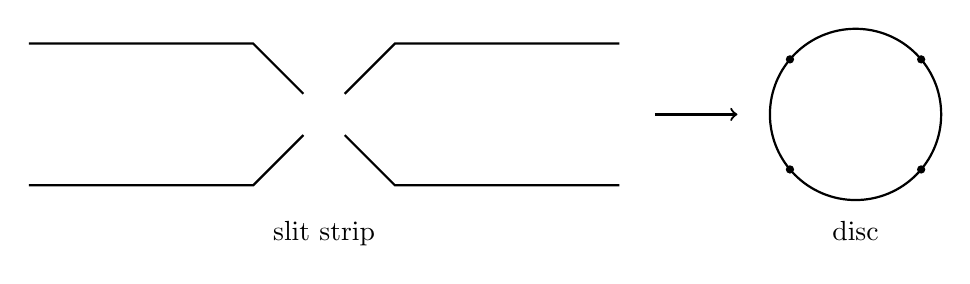
\begin{tikzpicture}[x=0.75cm,y=0.75cm]
    \draw[thick] (-5,1.2) -- (-1.2,1.2) -- (-0.35,0.35);
    \draw[thick] (-5,-1.2) -- (-1.2,-1.2) -- (-0.35,-0.35);
    \draw[thick] (0.35,0.35) -- (1.2,1.2) -- (5,1.2);
    \draw[thick] (0.35,-0.35) -- (1.2,-1.2) -- (5,-1.2);
    \draw[->,thick] (5.6,0) -- (7.0,0);
    \draw[thick] (9.0,0) circle (1.45);
    \foreach \a in {40,140,220,320} \fill (9.0,0) ++(\a:1.45) circle (1.5pt);
    \node[below] at (0,-1.65) {slit strip};
    \node[below] at (9.0,-1.65) {disc};
  \end{tikzpicture}
  \end{adjustbox}
  \caption{黑板上的等值線比較，以及將帶縫長帶共形映射至圓盤的清晰示意圖。四個外部端點映成四個特殊的邊界點。}
  \lectureframe{01:04:46}
  \label{fig:l07-strip-to-disc}
\end{figure}

改變座標並不會讓外部態消失。動量、粒子種類和振子能階都必須插入四個特殊點。承載這些資訊的形式物件稱為頂點算符。雖然其詳細構造留待後續討論，它們的作用已很清楚：將原本均勻的世界面路徑積分，轉化為指定的散射實驗。

利用圓盤的共形變換，將三個邊界點移至方便的參考位置後，還會剩下一個實數的相對位置。這個位置可用四個依序排列的邊界點之交比表示。它就是原先存續時間\(\tau_0\)在圓盤上的對應量。

\begin{figure}[H]
  \centering
  \includegraphics[width=0.62\textwidth]{lecture_07_figure_13.png}
  \caption{圓盤邊界上的四個插入點。共形自由度可消去其有序配置中除一個實模數外的所有模數。}
  \lectureframe{01:10:55}
  \label{fig:l07-four-points}
\end{figure}

因此，存續時間的積分並未消失，而是轉為對剩餘模數積分。採用慣用座標\(0<z<1\)時，四點開弦積分與上一講所得的形式相同：
\begin{equation}
  \mathcal A(s,t)\propto
  \int_0^1 z^{-s-1}(1-z)^{-t-1}\,dz.
  \label{eq:l07-modulus-integral}
\end{equation}

\section{同一曲面的兩種極限}

在模空間的一端，與入射粒子對應的兩個插入點彼此靠近。在帶縫長帶的座標中，這代表接合與分裂之間有一段很長的間隔：直接道中的中間弦會長時間傳播。在另一端，另一對相鄰插入點彼此靠近。此時，同一曲面自然可解讀為交叉道交換。這兩種描述在長帶圖像中看似毫不相關，卻是同一圓盤積分在相鄰邊界處的極限。

回到上一講採用的 mostly-plus 慣例，
\begin{equation}
  -s=(k_1+k_2)^2,
  \qquad
  -t=(k_1+k_3)^2.
  \label{eq:l07-mandelstam}
\end{equation}
直接道極限中的極點由\(s\)組織；交叉道極限中的極點則由\(t\)組織。
\editorialnote{講座接近尾聲時，黑板以簡寫符號表示曼德斯塔姆不變量，同時將\(s\)認定為正的質心系能量平方。方程\eqref{eq:l07-mandelstam}沿用第6講確立的 mostly-plus 慣例。}

\begin{figure}[H]
  \centering
  \includegraphics[width=0.62\textwidth]{lecture_07_figure_14.png}
  \caption{兩種道的圖示：一種取向呈現長時間傳播，交叉取向則呈現交換。}
  \lectureframe{01:19:27}
  \label{fig:l07-channel-diagrams}
\end{figure}

\begin{figure}[H]
  \centering
  \includegraphics[width=0.72\textwidth]{lecture_07_figure_15.png}
  \caption{黑板再次列出\(s\)道與\(t\)道的動量配對，並比較圓盤模數的兩個極限。}
  \lectureframe{01:19:40}
  \label{fig:l07-st-board}
\end{figure}

因此，同一個解析函數提供了兩種展開：
\begin{equation}
  \mathcal A(s,t)=\mathcal A(t,s).
\end{equation}
這就是道對偶。在最初以共振描述的脈絡中，對直接道態求和竟然也能編碼交叉道交換，曾令人覺得不可思議。在歐幾里得世界面上，共形對稱性解釋了為什麼兩種描述屬於同一個曲面。歷史上，這種詮釋在1969年維內齊亞諾振幅問世後不久便出現了。

\begin{classroomqa}
\audiencequestion{交叉取向是否也有相應的帶縫長帶圖像？\lecturetimestamp{01:20:49}}
\lecturerresponse{有，但必須以不同方式選取稱為時間的方向。同一個歐幾里得曲面可以採用另一種切片方式，讓另一對外部端點分別位於遙遠的過去與未來。正因為可以如此切片，單一世界面才有多種道的詮釋。}
\end{classroomqa}

\begin{classroomqa}
\audiencequestion{弦接合的時間長短由耦合常數決定嗎？\lecturetimestamp{01:21:39}}
\lecturerresponse{不會選定某個固定的存續時間。存續時間是積分變數，每個取值都會有所貢獻。耦合常數控制接合與分裂的權重---，也就是衰變強度---，並以乘法因子進入振幅；它不會取代對模數的積分。}
\end{classroomqa}
